\documentclass{article}
\usepackage[utf8]{inputenc}
\usepackage[english]{babel}
\usepackage{amsmath,amsfonts,amssymb,amsthm}
\usepackage{mathtools}
\usepackage{fancyhdr}
\usepackage{commath}
\usepackage[sc,osf]{mathpazo}
\usepackage{graphicx}
\usepackage{rotating}
\usepackage{float}
\usepackage{subcaption}
\restylefloat{table}
\usepackage{multicol}
\usepackage[dvipsnames]{xcolor}
\usepackage[colorinlistoftodos]{todonotes}
\usepackage{vmargin}  % Administrar márgenes
\setpapersize{A4} % Definir tamaño del papel
\setmargins{2.5cm} % Margen izquierdo
{1cm} % Margen superior
{16.5cm} % Área de impresión horizontal
{23.42cm} % Area de impresión vertical
{15mm} % Encabezado
{5mm} % Espacio entre el encabezado y el texto
{10pt} % Pie de página
{3mm} % Espacio entre el pie de página y el texto

\pagestyle{fancy}
\fancyhf{}
\rhead{

\includegraphics[width=4cm,height=1cm]{cropped-iitpal-at-prutor-logo.png}
}
\lhead{Determinants | Class XII}
\rfoot{}
\begin{document}
\section{Consistency and Inconsistency}
A system of linear equations having two and three variables can be easily solved using determinants. When system of equations has at least one solution it is called consistent, and if there are no solutions at all then it is called inconsistent. Below diagram clearifies,
\begin{figure}[H]
    \centering
    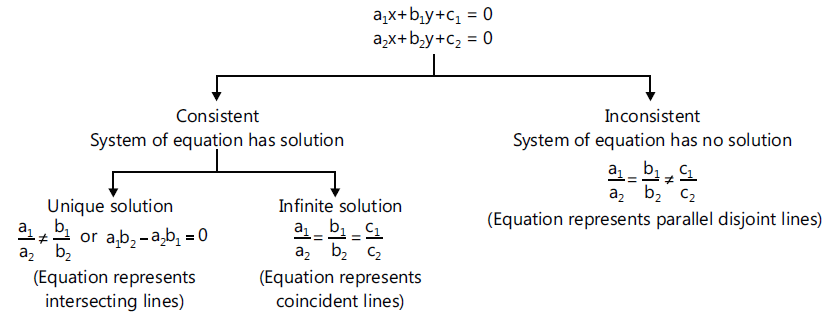
\includegraphics[scale=0.5]{determinants_lec4_notes-1.png}
\end{figure}
\section{Cramer's Rule}
For 3 linear equations system,
\begin{align*}
    a_1x+b_1y+c_1z=d_1\\
    a_2x+b_2y+c_2z=d_1\\
    a_3x+b_3y+c_3z=d_1\\
\end{align*}
Define following determinants,
\begin{equation*}
    \Delta=
    \begin{vmatrix}
        a_1 & b_1 & c_1 \\
        a_2 & b_2 & c_2 \\
        a_3 & b_3 & c_3 \\
    \end{vmatrix}
\end{equation*}
\begin{equation*}
    \Delta_1=
    \begin{vmatrix}
        d_1 & b_1 & c_1 \\
        d_2 & b_2 & c_2 \\
        d_3 & b_3 & c_3 \\
    \end{vmatrix},
    \Delta_2=
    \begin{vmatrix}
        a_1 & d_1 & c_1 \\
        a_2 & d_2 & c_2 \\
        a_3 & d_3 & c_3 \\
    \end{vmatrix},
    \Delta_3=
    \begin{vmatrix}
        a_1 & b_1 & d_1 \\
        a_2 & b_2 & d_2 \\
        a_3 & b_3 & d_3 \\
    \end{vmatrix}
\end{equation*}
Now Cramer's rule gives solution when $\Delta \neq 0$
\begin{equation*}
    x=\frac{\Delta_1}{\Delta},y=\frac{\Delta_2}{\Delta},z=\frac{\Delta_3}{\Delta}
\end{equation*}
\section{Conditions for Infinite and No Solutions}
\begin{figure}[H]
    \centering
    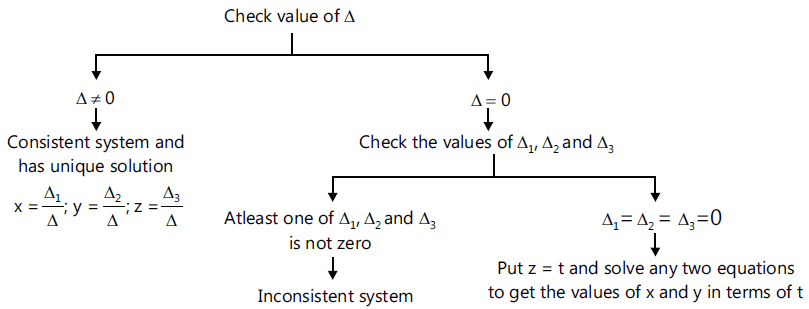
\includegraphics[scale=0.5]{determinants_lec4_notes-2.png}
\end{figure}
\paragraph{Points}
\begin{enumerate}
    \item If $\Delta \neq 0$ then the given system of equations are
    consistent and have unique solution.
    \item If $\Delta = 0$ but at least one of $\Delta_1, \Delta_2 , \Delta_3$ is not zero then
    the equations are inconsistent and have no solution.
    \item If $\Delta_1=\Delta_2 = \Delta_3=\Delta=0$ then the given system of equations are consistent and have infinite solution
    except the case of parallel planes when there is no
    solution. 
\end{enumerate}
\section{Homogeneous Linear Equations}
If ${{d}_{1}}={{d}_{2}}={{d}_{3}}=0$, then system of linear equations is known as Homogeneous linear equations, which always possess at least one solution i.e. (0, 0, 0). This is called a trivial solution for homogeneous linear equations.
\begin{enumerate}
    \item Solution of Homogenous Equations is always
    consistent, as $x = 0 = y = z$ is always a solution.
    This is known as TRIVIAL solution.
    \item  For Homogenous Equations, if $\Delta \neq 0$. Then
    $x = 0 = y = z$ is only solution.    
    \item  For Homogenous Equations, if $\Delta = 0$, then there exists
    non zero solutions (\textbf{NON TRIVIAL SOLUTIONS}) also.    
\end{enumerate}
\end{document}